% -------------------------------------------------------------------------------------- %

\section{Appendix}

When $N \geq M$ and the kernel has orthogonal features, 
\begin{equation}
    P = \Sigma^{-2} \widehat{ K }^* \Sigma^2
\end{equation}

\subsection{Transfer Operator for Blaschke Products}

We consider the analytic mapping on the unit circle in $\bbC$, 
\begin{equation*}
    \tau : \bbT \circlearrowleft, \quad z \mapsto z \frac{z - \mu}{1 - \bar{\mu} z} 
\end{equation*}
dependent on a parameter $\mu \in \bbD$ in the open unit disk. 

$\tau$ is a Lebesgue-measure preserving 2-to-1 map. The spectrum 
$\sigma \left( \scrK \vert_{L^2 (d\theta)} \right) = \overline{\bbD}$ is the whole unit 
disk, point spectrum 
$\sigma_p \left( \scrK \vert_{L^2 (d\theta)} \right) = \left\{ 1 \right\}$. 

When considering instead the adjoint $\scrL = \scrK^*$, the point spectrum has the 
interesting property that 
$\left\{ \mu^k \right\}_{k=0}^\infty \cup \left\{ \overline{\mu}^k \right\}_{k=0}^\infty \subset \sigma_p \left( \scrL \vert_{L^2 (d\theta)} \right)$. 

More specifically, let $\bbT \subset A$ be a (suitably chosen) open annulus containing the 
unit circle, and $H^2 (A)$ be the Hardy Hilbert space of holomorphic functions on $A$ which 
are square integrable on the edge $\partial A$. Then on this space, 
$\sigma \left( \scrL \vert_{H^2 (A)} \right) = \left\{ \mu^k \right\}_{k=0}^\infty \cup \left\{ \overline{\mu}^k \right\}_{k=0}^\infty$. 

EDMD with monomials $\left\{ z \mapsto z^k \right\}_{k=-N}^N$ (Fourier basis) results in 
eigendecompositions which converge exponentially to 
$\sigma \left( \scrL \vert_{H^2 (A)} \right)$ as $N \to \infty$. 


\begin{figure}
    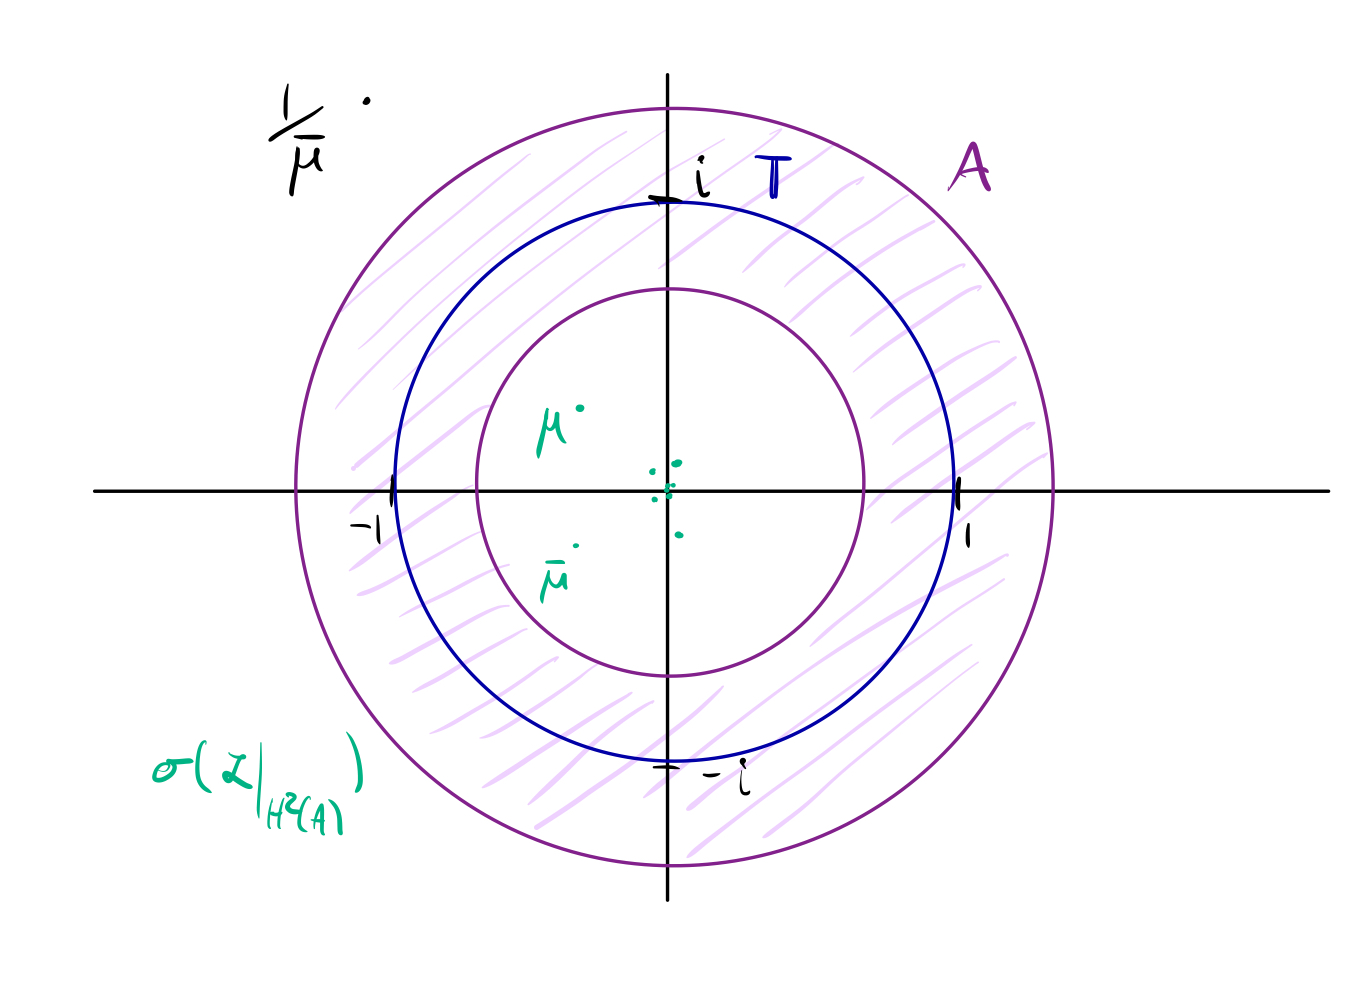
\includegraphics[width=\textwidth]{H2A.jpeg}
    \caption{
        Unit circle $\bbT$ and Annulus $A$. 
    }
\end{figure}

\begin{figure}
    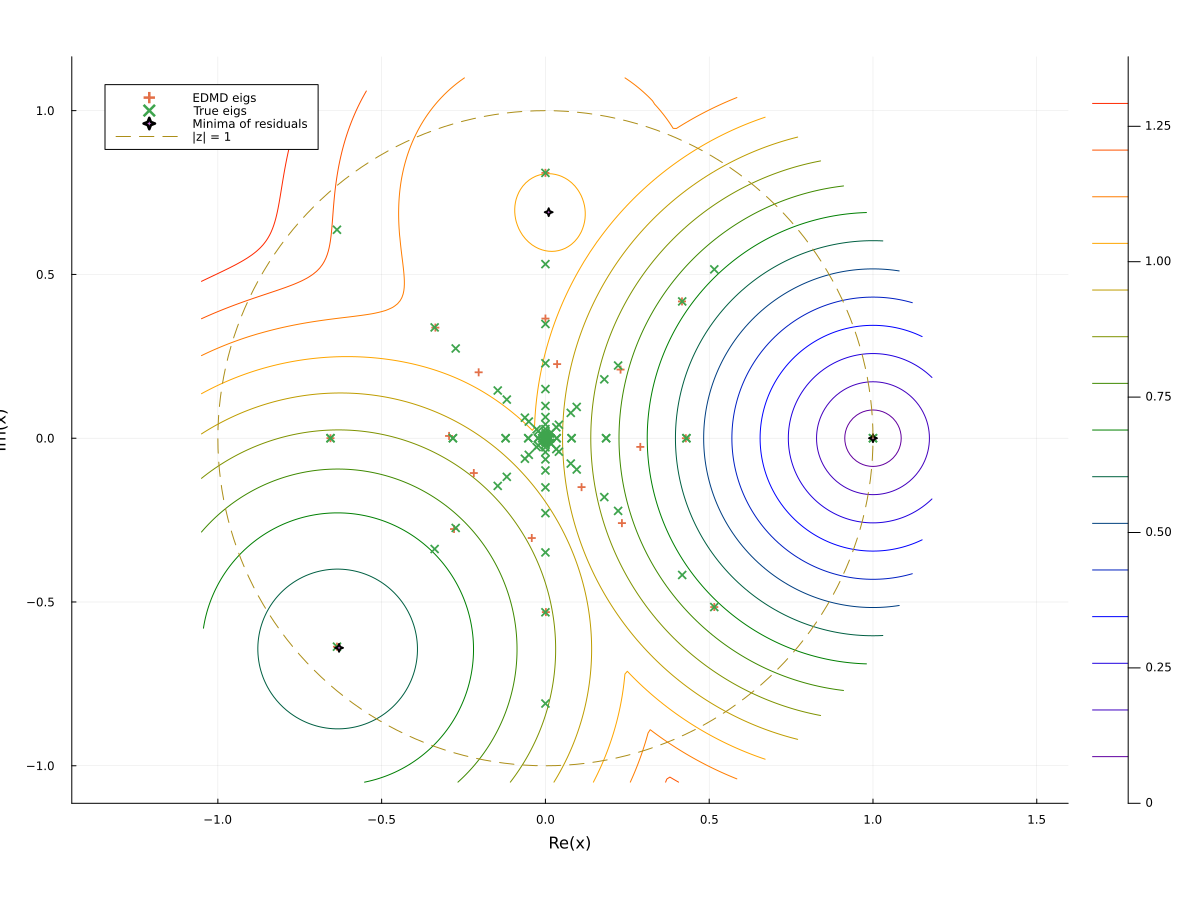
\includegraphics[width=\textwidth]{resdmd.png}
    \caption{
        ResDMD over the space $L^2(\bbT)$ for a Blaschke map 
        $\tau (z) = z \frac{z - \mu}{1 - \bar{\mu} z}$ with $\mu = 0.9 e^{\pi i / 4}$. 
        True eigenvalues are known in the Hardy space $H^2 (A)$ of functions holomorphic on 
        the annulus 
        $A = \left\{ z \in \mathbb{C} \mid r < |z| < R \right\}$, 
        $R = 11/10 - 1/32$, $r = 1/R$. ResDMD matrices $G, A, L$ are computed w.r.t. this   
        Hilbert space, using a dictionary of $N = 20$ monomials and $M = 200,000$
        equally spaced quadrature nodes. 
    }
    \label{fig:resdmd}
\end{figure}

\begin{figure}
    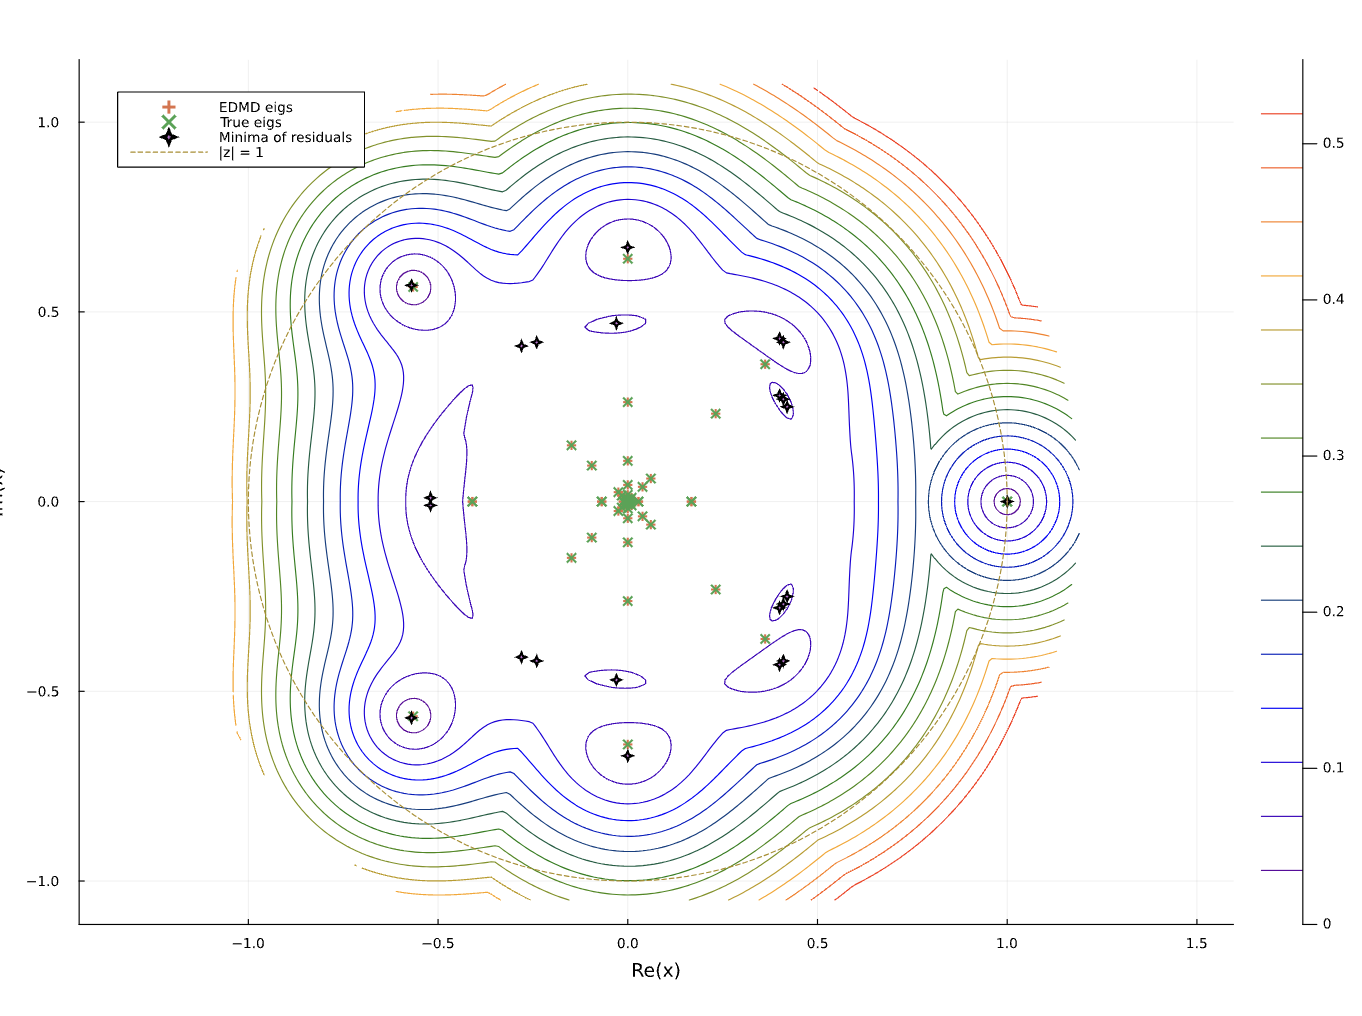
\includegraphics[width=\textwidth]{H2AC_resdmd.png}
    \caption{
        ResDMD for $\mu = 0.8 e^{\pi i / 4}$ over the space $H^2 (A)^*$, where 
        $H^2 (A) \subset L^2$ is seen as embedded in $L^2$ and $(\cdot)^*$ the Banach space 
        adjoint. This dual space is isomorphic to the space 
        $H^2 (\bbD_r) \oplus H^2 (\bbD_{1/r}^\infty)$ and has a norm 
        $\| f \|_{H^2 (A)^*}^2 = \sum_{n \in \bbZ} | \hat{f} |^2 r^{| n |}$. 
    }
\end{figure}

\begin{figure}
    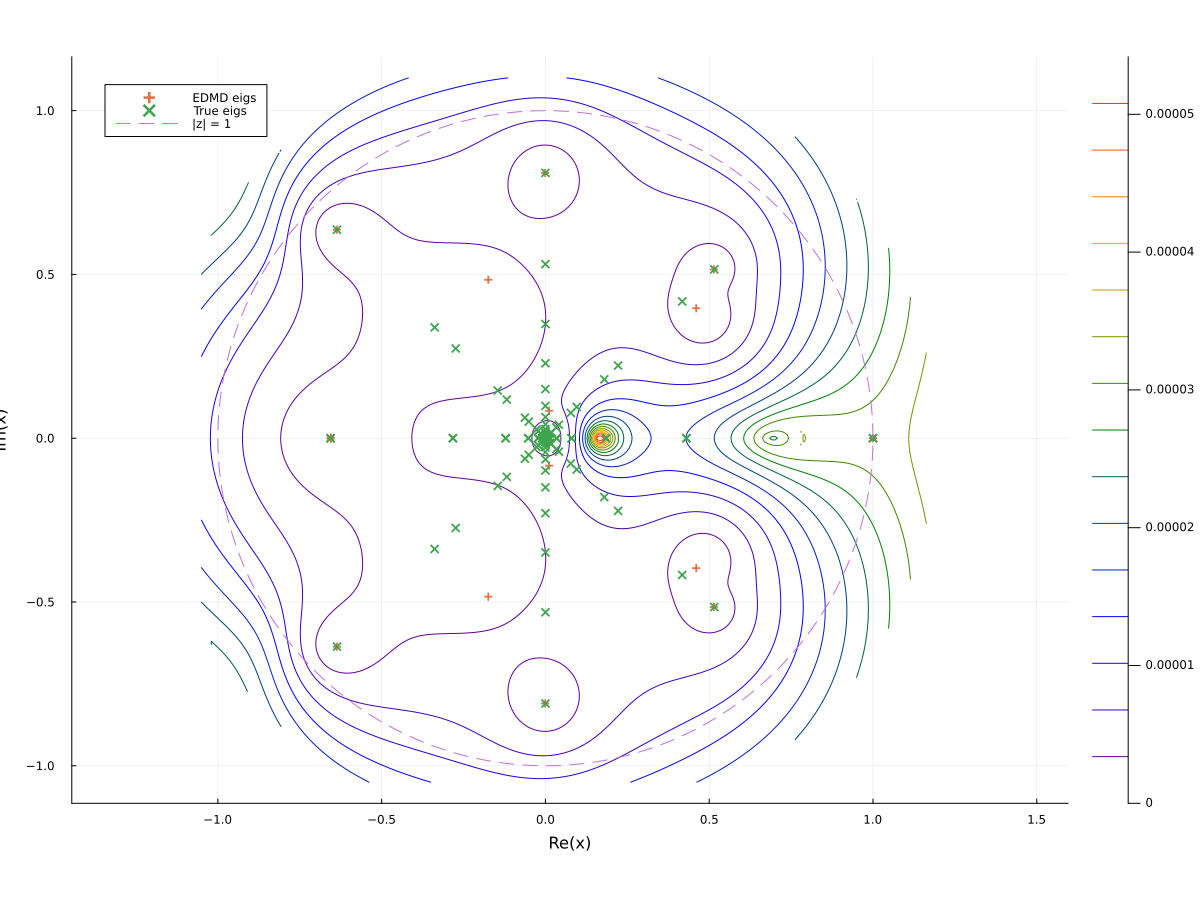
\includegraphics[width=\textwidth]{polynomial_kresdmd.png}
    \caption{
        Kernelized ResDMD for the Blaschke map using a degree $20$ polynomial kernel 
        $k(x,y) = (1 + x'y)^{20}$ 
        and $M = 2,000$ equally spaced quadrature nodes. 
    }
    \label{fig:poly}
\end{figure}

\begin{figure}
    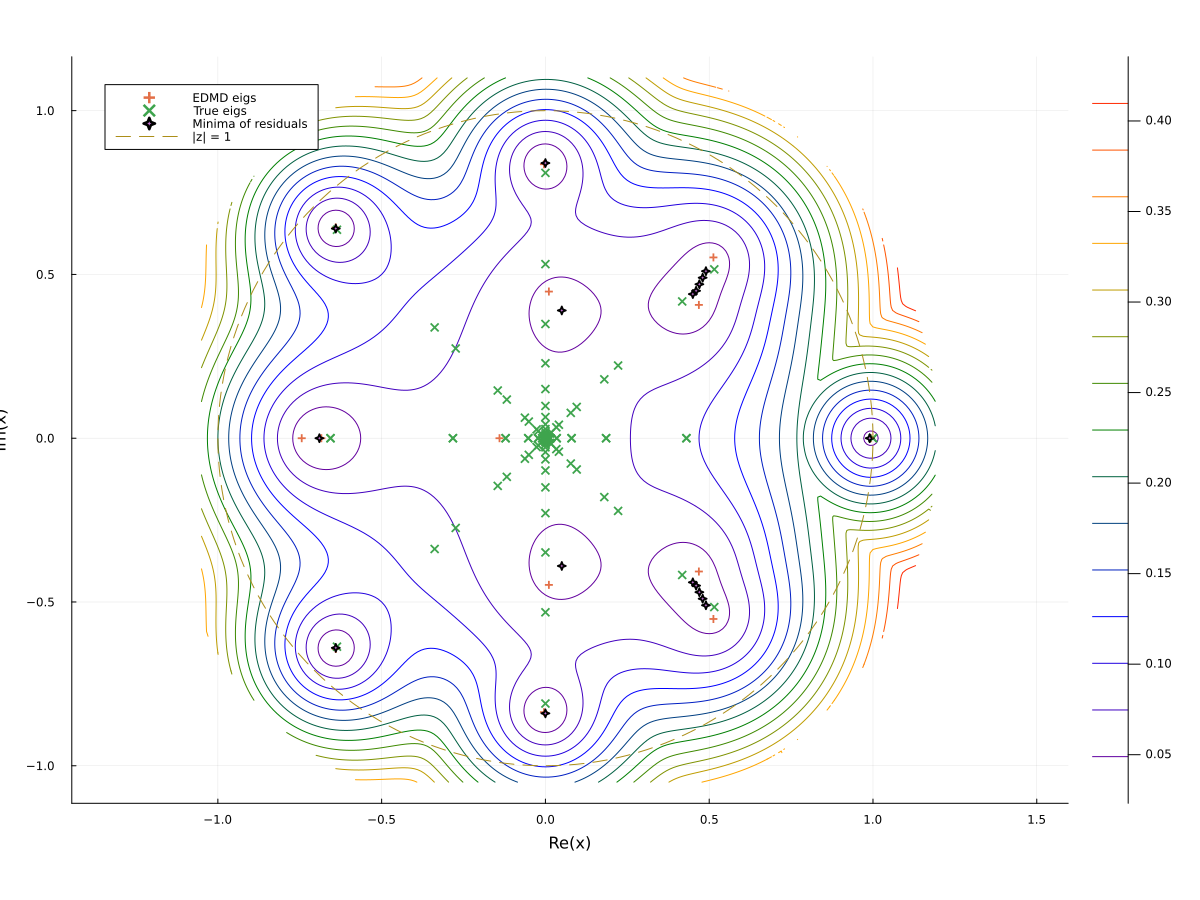
\includegraphics[width=\textwidth]{rbf_kresdmd.png}
    \caption{
        Kernelized ResDMD using an RBF kernel $k(x,y) = e^{- |x - y|^2 / c}$ with 
        $c = 0.01$ and $M = 2,000$ equally spaced quadrature nodes. 
    }
    \label{fig:gauss}
\end{figure}


\subsection{Some scribbles about kernels and residuals}

\textbf{EDMD:} EDMD is a Petrov-Galerkin method as written in Péter's 2016 paper. 
Considering a dictionary $\left\{ \psi_i \right\}_{i=1}^N \subset \scrH$ ($\scrH = L^2$ 
mostly) and snapshots $\left\{ x_j \right\}_{j=1}^M \subset X$, EDMD makes the following 
construction:

\begin{equation}
    \Psi (x) = \left[ \psi_1 \ldots \psi_N \right]
\end{equation}

We find a matrix $K \in \bbC^{N \times N}$ that minimizes

\begin{equation}
    \label{L2min}
    \| \scrK \Psi - \Psi K \|_{\scrH (X, \bbC^{1 \times N})}
\end{equation}

The $\scrH$ norm is approximated by a quadrature:

\begin{equation}
    \YX = \Psi 
        \begin{pmatrix}
            x_1 \\
            \vdots \\
            x_M
        \end{pmatrix}
    , \quad
    \YY = \Psi \circ S 
        \begin{pmatrix}
            x_1 \\
            \vdots \\
            x_M
        \end{pmatrix}
\end{equation}

\begin{equation}
    \label{l2min}
    \| \scrK \Psi - \Psi K \|_{\scrH (X, \bbC^{1 \times N})}
    \approx
    \| \YY - \YX K \|_F . 
\end{equation}

\ref{L2min} is minimized by 

\begin{equation}
    K = \YX^\dagger \YY = G^\dagger A
\end{equation}

where $G = \YX^* \YX$, $A = \YX^* \YY$. 

\textbf{EDMD for Perron-Frobenius:} Since

\begin{equation}
    A_{i j} \stackrel{M \to \infty}{\approx} \left\langle \psi_i, \scrK \psi_j 
    \right\rangle = 
    \left\langle \scrL \psi_i, \psi_j \right\rangle, 
\end{equation}

an equivalent Galerkin approximation for $\scrL = \scrK^*$ is given by

\begin{equation}
    P = G^\dagger A^* = \YX^\dagger {\YX^*}^\dagger \YY^* \YX . 
\end{equation}

\textbf{kEDMD:} Let $k : X \times X \to \bbC$ be a kernel so that 

\begin{equation}
    k(x_i, x_j) = \left\langle \Psi (x_i), \Psi (x_j) \right\rangle_{\ell^2}\ \left(\, = 
    \Psi (x_i) \Psi (x_j)^* \,\right) .
\end{equation}

( Note that $\Psi (x)$ might be infinite-dimensional, i.e. $N = \infty$, but we think of 
$N < \infty$ for clarity of the matrix manipulations. )

Let further $\YX \stackrel{\text{SVD}}{=} Q \Sigma Z^*$ and

\begin{equation}
    \hat{G} = \left( k(x_i, x_j) \right)_{i j} = 
    \YX \YX^* 
    \stackrel{\text{diagonalize}}{=} Q (\Sigma^* \Sigma) Q^*, 
\end{equation}

\begin{equation}
    \hat{A} = \left( k(y_i, x_j) \right)_{i j} = 
    \YY \YX^*
\end{equation}

Then 

\begin{equation}
    \hat{K} = ( \Sigma^\dagger Q^* ) \hat{A} ( Q \Sigma^\dagger ) \in \bbC^{M \times M}
\end{equation}

has the same eigenvalues as $K$. 

\textbf{ResDMD:} The key idea behind ResDMD is, for an element $z \in \bbC^N$, 
$g = \Psi z$: 

\begin{align}
    \res (\lambda, z) &:= 
    \| (\scrK - \lambda) g \|_{\scrH (X, \bbC)}^2 \\
    &\stackrel{M \to \infty}{\approx} \| (\YY - \lambda \YX) z \|_{\ell^2}^2 \\
    &= z^* \left( \YY^* \YY - \lambda \YY^* \YX - \overline{\lambda} \YX^* \YY + 
    | \lambda |^2 \YX^* \YX \right) z \\
    &= z^* (L - \lambda A^* - \overline{\lambda} A + | \lambda |^2 G) z . 
\end{align}

We interpret the first equation as 

\begin{equation}
    \label{idea}
    regression\ error \stackrel{M \to \infty}{\approx} operator\ residual .
\end{equation}

The function $\lambda \mapsto \res (\lambda) = \min_z \res (\lambda, z)$ is shown in 
\ref{fig:resdmd}

\textbf{kResDMD:} We apply idea \ref{idea} to $\hat{K}$: 

\begin{equation}
    \hat{K}^* = \left( \YX^* Q \Sigma^\dagger \right)^\dagger 
    \left( \YY^* Q \Sigma^\dagger \right) =:
    \hat{\YX}^\dagger \hat{\YY}
\end{equation}

so that $\hat{K}^*$ solves the regression problem

\begin{equation}
    \min_M \| \hat{\YY} - \hat{\YX} M \|_F . 
\end{equation}

The regresion error reduces to

\begin{align}
    \hat{\res} (\lambda, z) 
    &:= \| ( \hat{\YY} - \lambda \hat{\YX} ) z \|_{\ell^2}^2 \\
    &= (Q \Sigma^\dagger z)^* \left( 
        \YY \YY^* 
        - \lambda \YY \YX^* 
        - \overline{\lambda} \YX \YY^* 
        + | \lambda |^2 \YX \YX^*
    \right) (Q \Sigma^\dagger z) \\
    &= (Q \Sigma^\dagger z)^* \left( 
        \hat{L}
        - \lambda \hat{A}^*
        - \overline{\lambda} \hat{A}
        + | \lambda |^2 \hat{G}
    \right) (Q \Sigma^\dagger z)
\end{align}

Note at this point it is unclear whether this regression error in the case of $\hat{K}$ 
has a physical meaning. 

\textbf{ResDMD for Perron-Frobenius:} Consider $\tilde{P} = Z^* P Z$, which has the same 
eigenvalues as $P$. Then 

\begin{equation}
    \tilde{P} = \left( \YX^* Q \Sigma \right)^\dagger \left( \YY^* Q \Sigma \right) =:
    \tilde{\YX}^\dagger \tilde{\YY}
\end{equation}

so that $\hat{P}$ solves the regresion problem

\begin{equation}
    \min_M \| \tilde{\YY} - \tilde{\YX} M \|_F . 
\end{equation}

The interesting thing to note is that 

\begin{align}
    \tilde{\res} (\lambda, z)
    &:= \| ( \tilde{\YY} - \lambda \tilde{\YX} ) z \|_{\ell^2}^2 \\
    &= (Q \Sigma z)^* \left( 
        \YY \YY^* 
        - \lambda \YY \YX^* 
        - \overline{\lambda} \YX \YY^* 
        + | \lambda |^2 \YX \YX^*
    \right) (Q \Sigma z) \\
    &= (Q \Sigma z)^* \left( 
        \hat{L}
        - \lambda \hat{A}^*
        - \overline{\lambda} \hat{A}
        + | \lambda |^2 \hat{G}
    \right) (Q \Sigma z)
\end{align}

and hence whenever $\YX$ has the same number of zero singular values (we assume there 
are none i.e. $s_{min} (\YX) > 0$),

\begin{equation}
    \hat{\res} (\lambda) := \min_z\ \hat{\res} (\lambda, z) 
    = \min_\xi\ \tilde{\res} (\lambda, \xi) =: \tilde{\res} (\lambda) . 
\end{equation}

The function $\hat{\res}$ is shown in \ref{fig:poly}, \ref{fig:gauss}. 

\textbf{Interpreting the regression error:} Let $y = Q \Sigma z$. For convenience we 
conjugate $\lambda$, i.e. let $\tilde{P} z = \overline{\lambda} z$ be a candidate 
eigenpair for $\scrL$. 

What follows is a rough, purely formal sketch of the idea that we want to show, 
from what I calculated this morning (no promises for correctness):

\begin{align}
    &\| (\YY^* - \overline{\lambda} \YX^*) y \|_{\ell^2}^2 \\
    &= \sum_{i=1}^N \left|\ 
        \sum_{j=1}^{M} \overline{(\scrK \psi_i - \lambda \psi_i) (x_j)}\ y_j
     \ \right|^2 \\
    &\stackrel{M \to \infty}{\approx} 
     \sum_{i=1}^{N} \left|\ 
        \int \overline{(\scrK \psi_i - \lambda \psi_i) (\xi)}\ y (\xi)\ d\xi
     \ \right|^2 \label{limfunc} \\
    &= \sum_{i=1}^{N} \left| \left\langle (\scrK - \lambda) \psi_i,\, y \right\rangle \right|^2 \\
    &= \sum_{i=1}^{N} \left| \left\langle \psi_i,\, (\scrL - \overline{\lambda}) y \right\rangle \right|^2 \\
    &\stackrel{N \to \infty}{\approx}
     \| (\scrL - \overline{\lambda}) y \|_{\scrH (X, \bbC)}^2 . \label{plancherel}
\end{align}

where for \ref{limfunc} we say that the vector $y = (y_j)_j$ converges to a function 
$y : \xi \mapsto y (\xi)$, and for \ref{plancherel} we use Plancherel's theorem (hence 
we need to assume $\Psi$ is an orthonormal family that in the limit has span dense in 
$\scrH(X, \bbC)$). 

It seems likely that these convergences will work, under the crucial assumption that 
the singular values stay bounded from above and below as $N \to \infty$, which  is given 
if $\Psi$ is an orthonormal family. There is some literature on kernel $QR$ algorithms, 
which are essentially Gram-Schmidt for kernel weight matrices. However, I would much 
prefer if this would work without the orthonormal requirement, as most kernel functions 
and snapshot datasets will not make orthonormal Gram matrices. 

For e.g. Gauß kernels $k(x,y) = \exp (- \| x - y \|^2 / c)$, the sharpness parameter $c$ 
has to be changed as $M$ changes in order for the singular value condition to hold since 
if $c$ is kept constant and $M$ grows, the Gram matrix slowly becomes the all-ones matrix. 

\begin{figure}
    \centering 
    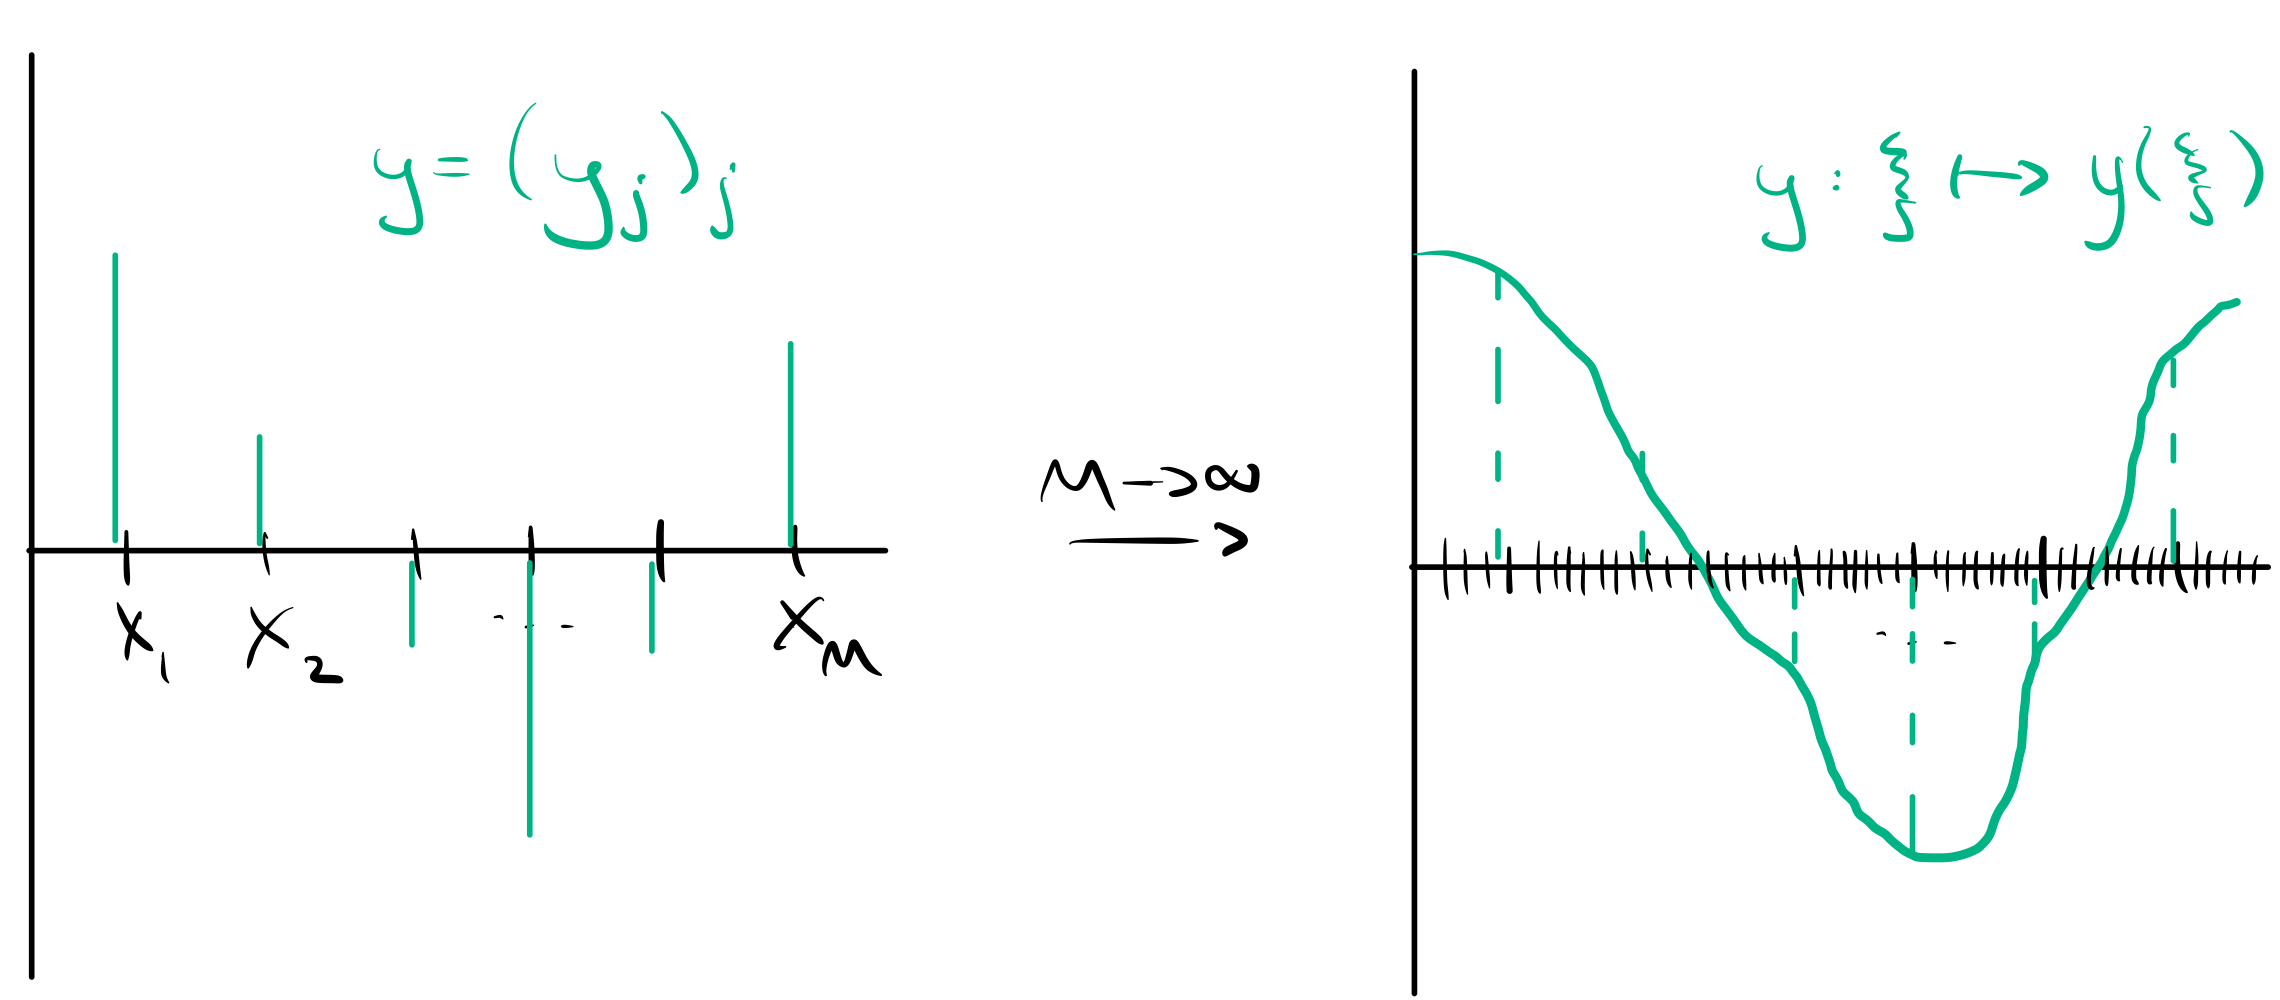
\includegraphics[width=\textwidth]{yfunction.jpeg}
    \caption{
        Idea behind equation \ref{limfunc}
    }
\end{figure}

% -------------------------------------------------------------------------------------- %
